\label{sec:transition}
\subsection{Why Transition?}
In order for the UAV to complete the objectives listed in Section \ref{sec:intro}, it must be capable of both long range flight and vertical take-off and landing. Implementing a transition system, rather than fit the UAV with both fixed-wing and VTOL flight systems, allows it to achieve this capability while also being lighter, and more aerodynamic. The transition systems is the foundation for achieving the range and endurance requirements of the UAV Challenge.

\subsection{Gyroscopic Forces}
An analysis of the gyroscopic forces acting on the motors during transition was performed to determine the required configuration of the motors, the strength of the shaft between the two motors, and the torque required to perform transition. The calculations (see Appendix  \ref{sec:gyro}) showed that by having the two front motors spinning in opposite directions, there is no resultant moment acting on the transition system. The front servo would therefore receive no counter moment in flight, and an arbitrary 8.65kg/cm (0.85Nm) servo was selected. In order to verify the servo could rotate the front motors during flight, the UAV was lashed down and the propellers throttled to full speed. The servo showed no signs of difficulty, and was successful in rotating the shaft at full throttle.\\

However, the carbon fiber pole experiences bending moments during transition that may result in fracture. The total moment created by the gyroscopic motion was calculated to be a maximum of 3.1Nm in the center of the shaft. Given the maximum rotation speed of the propellers, the moment generated by gravity acting on the shaft and motors during hover is ~9.156Nm, which is much greater than the gyroscopic force during transition. The transition system also needs to be able to withstand other gyroscopic forces, such as if the UAV rolls rapidly. In this case, a moment would be created on each of the motors, but due to the counter-rotating front motors, these forces would again negate each other. From this analysis it can also be concluded that after any transition or fast movements, these counteracting forces also act to eliminate any unwanted rotations of the aircraft caused by the gyroscopic moment. 

\subsection{System Design}
\label{sec:controller}
The transition system was implemented with a 1:1 3D printed gear system, fixed to a 3D printed mount which is fixed in the nose of the UAV, as shown in Figure \ref{fig:gearsys}. This allowed for full rotation of the servo, and maximum accuracy. Since the desired functionality was not available on the PixHawk, the open source PX4 firmware was expanded to have a new flight mode that enabled transition, requiring a detailed understanding of both the PixHawk \cite{ref:firmware1} and the open source ArduPilot \cite{ref:firmware2} project.

\begin{figure}[!ht]
	\centering
	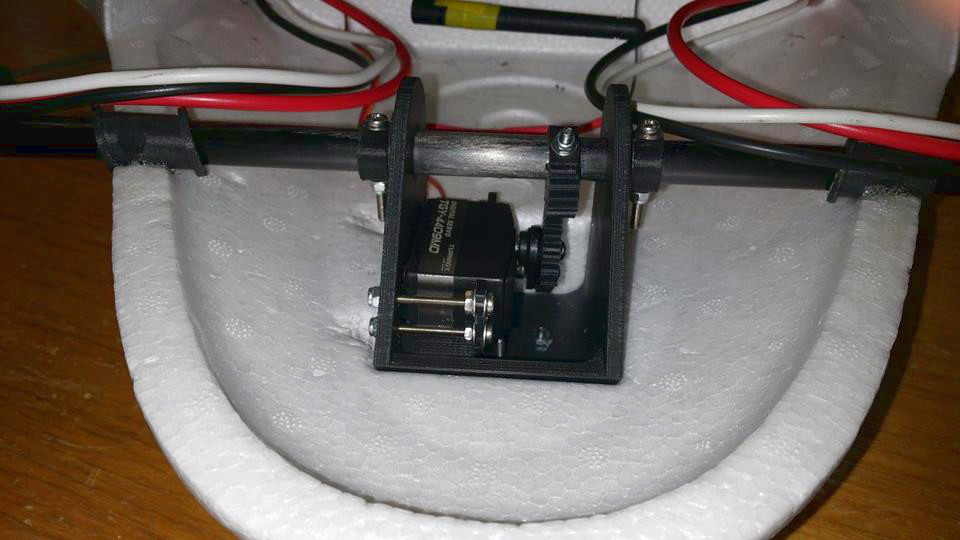
\includegraphics[width=300pt]{\IMAGEPATH /Prototype/gear_system}
	\caption{Front gear and mounting system}
	\label{fig:gearsys}
\end{figure}

The new flight mode is currently only configured for manual flight using an RC transmitter, rather than autonomous flight. When a switch on the RC transmitter is toggled the flight controls are converted from VTOL flight to fixed-wing, and the transition system activates, rotating the front motors forward 90$^\circ$. In order for the flight control conversion to work, the firmware was also modified so that after transition, the RC controls no longer affect the rotation of the UAV, but now control its fixed-wing control surfaces (such as the ailerons). Further firmware developments will be required in order to achieve stable, autonomous flight.\\

\subsection{Testing}
Given that the UAV must currently be transitioned manually, \cite{ref:fireflyinstruction} suggests a sequence of steps to perform to achieve successful transition into fixed wing mode: 
\begin{itemize}
\item While in altitude hold mode, keep the throttle at 50\% and move the aircraft forward to generate speed
\item Toggle the transition switch 
\item Lower the throttle
\item Pull up and raise the throttle as required		
\end{itemize}

Off-line tests were conducted with the Dragonfly prototype to practice this procedure; the UAV was held down and the front motors transitioned while the motors were spun at hover speed. After transition, the UAV's control surfaces behaved as expected, and a successful transition simulation was achieved. Unfortunately, due to weather and other factors described in Table \ref{tab:tests}, the transition system testing was not completed at the writing of this report.
